\chapter{Error computation\label{chap:error}}

This chapter presents the different methods for computing the error field associated to the analysis, as well as the error resulting from the calculation of the integral of a field over a domain.

\minitoc

%------------------
\section{Introduction}
%------------------

The analysis performed with the optimised parameters should have the lowest global error, as measured by \eqref{eq:gcvbis}. Nevertheless, the spatial distribution of the error is also of interest for any interpolation or analysis method, since it gives the user an indication of the reliability of the results. The error field is expected to be affected by:
\begin{enumerate}
\item the data coverage: the error field is expected to be higher where the data coverage is lower;
\item the noise on the data: the more uncertainties we have on the data, the higher will be the error field.
\end{enumerate}


OI (Sections~\ref{sec:OImethod}) \index{OI} allows the simultaneous derivation of analysis and error fields:
\be
e^{2}(\mathbf{r}) = \sigma^{2}(\mathbf{r})-\transp{\mathbf{g}(\mathbf{r})}\mathbf{D}^{-1}  \mathbf{g}(\mathbf{r}),
\label{eq:erroroi}
\ee
where $\sigma^{2}$ is the local variance of the background field. This equality highlights that the error is provided by the analysis of a pseudo-data array containing covariances\index{Covariance} $\mathbf{g}(\mathbf{r})$. 

However, in principle, a new analysis has to be performed for each point $\mathbf{r}$ in which the error is requested and then is not adapted for large data sets. On the contrary, the error calculation in \diva is not trivial since the covariance functions are never explicitly specified. We will see in the next sections how \diva computes this error field.

%-------------------------------------

According to the data sets, the type of analysis (with/without dynamical constraints, constant or variable correlation length, \ldots), several error calculation methods are available with \diva. 

\subsection{The poor man's estimate\label{sec:poormans}}
%-------------------------------------------------------

To circumvent the main problems (unknown covariance function and repeated analysis), \citet{BRASSEUR94} estimated the error by analysing a vector of "covariances" with constant $\sigma^2$. As all covariances are identical, the error can be assessed in all locations with the same analysis. The advantage is the fast calculation, but the drawback is a systematic underestimation of the actual errors, since the error reduction by the overestimated covariances \eqref{eq:erroroi} is also overestimated. The poor man's error field is a very efficient way to assess data-coverage and determine the regions where the analysis cannot be trusted.

\subsection{The clever poor man's estimate\label{sec:cleverpoormans}}

Compared to the poor man's estimate, this approach still analyses a vector of "covariances" with constant $\sigma^2$ but reduces the correlation length so that for isolated observations, the resulting error field is almost exact. When data points are closer to each other (typically within the range of the correlation length), then the methods is still to optimistic.

{\it more to come}

\subsection{The hybrid approach}
%-------------------------------

In this approach, \citet{BRANKART98} and \citet{RIXEN00} proposed a heuristic statistical error expression for the VIM: in \diva, error fields are calculated by analogy with OI: since analysis in OI is equivalent to analysis with VIM (insofar as the reproducing Kernel of VIM and the covariance function of OI are identical) and since error field of OI equals analysis of covariance fields, error field of VIM equals analysis (by VIM) of covariance fields.\index{VIM}

Mathematically, according to the developments of Section~\ref{sec:OImethod}, we have:

\begin{align}
\textrm{Solution OI:} 	&	& \varphi(\mathbf{r}) &=& \underbrace{\mathbf{g}\transp{(\mathbf{r})}\mathbf{D}^{-1}}_{(\star)}		&& \mathbf{d}\\
\textrm{Solution VIM:}	&	& \varphi(\mathbf{r}) &=& \underbrace{\mathbf{T_{1}}(\mathbf{r})\mathbf{K}^{-1} \mathbf{T_{2}}(\mathbf{r})}_{(\star\star)} 																								&&\mathbf{d}\\
\textrm{Error~OI:}  	& 	& e^{2}(\mathbf{r})   &=& \sigma^{2}(\mathbf{r})-\underbrace{\mathbf{g}\transp{(\mathbf{r})}\mathbf{D}^{-1}}_{(\star)}														&&\mathbf{g}(\mathbf{r})	\\		
\rightarrow \textrm{Error~VIM:}		& 	& e^{2}(\mathbf{r})   &=& \sigma^{2}(\mathbf{r})-\underbrace{\mathbf{T_{1}}(\mathbf{r})\mathbf{K}^{-1} \mathbf{T_{2}}(\mathbf{r})}_{(\star\star)}		&&\mathbf{g}(\mathbf{r})
\end{align}

In practice, the data input of the analysis tool for an error calculation is a vector containing the
covariance of data points ($\mathbf{g}(\mathbf{r})$) with the point in which the error estimate is to be calculated. The covariance vector to be analysed is calculated using the correlation function (or Kernel\index{Kernel function}) $\mathbf{c}$ of an infinite domain in terms of the Bessel function as shown in \eqref{kernelfunction}:
\begin{equation}
e^{2}(\mathbf{r})   = \sigma^{2}(\mathbf{r})-\sigma^{2}(\mathbf{r}) \underbrace{\mathbf{T_{1}}(\mathbf{r})\mathbf{K}^{-1} \mathbf{T_{2}}(\mathbf{r})}_{(\star\star)}		\mathbf{c}(\mathbf{r})
\label{eq:kernelbessel}
\end{equation}
In an infinite domain, the error calculation is then "exact", while for more complicated domains, it is nearly exact far away from boundaries, provided no anisotropic constraint (advection constraint, variable length scale, boundaries, \ldots) is activated. 

Thus for anisotropic cases, the hybrid error field can provide incoherent results. This is what motivated the evaluation of the real covariance function in \diva.


\subsection{The real covariance method\label{sec:realcovariance}}
%--------------------------------------

If we look back at the OI interpretation, we can place a data of value $1$ at location $\vect{r}$ and compute the analysis $\varphi_1(\vect{r}^\prime)$ at a location $\vect{r}^\prime$:
\begin{equation}
\varphi_1(\vect{r}^\prime) = {\snr \hat{B} (\vect{r},\vect{r}^\prime)\over  \snr \hat{B}(\vect{r},\vect{r}) + \hat{R}(\vect{r}) },
\end{equation}
where $\hat{B}(\vect{r},\vect{r}^\prime)$ is the non-dimensional covariance function between points $\vect{r}$ and $\vect{r}^\prime$, whereas $\hat{R}$ is the normalized observational error variance. Normalization was done respectively by the background variance $\sigma^2$ and noise $\noise^2$, yielding the signal-to-noise ratio $\snr$ previously defined. 
At the data location itself, we get the analysis
\begin{equation}
\varphi_1(\vect{r}) = {\snr \hat{B} (\vect{r},\vect{r}) \over \snr \hat{B}(\vect{r},\vect{r}) + \hat{R}(\vect{r}) }.
\end{equation}

In terms of interpretation of the covariance function as the kernel of the norm (\eqref{divaformula2}), it is the background covariance that is modified by the anisotropy and not the noise level. Hence, if we put the unit data value with a unit signal-to-noise ratio in $\vect{r}$, we directly have

\begin{equation}
\varphi_1(\vect{r}^\prime) = { \hat{B} (\vect{r},\vect{r}^\prime)\over   \hat{B}(\vect{r},\vect{r}) + 1 } \qquad \textrm{and} \qquad 
\varphi_1(\vect{r}) = { \hat{B} (\vect{r},\vect{r}) \over  \hat{B}(\vect{r},\vect{r}) + 1 }.
\end{equation}
The left-hand sides are provided by the \diva application to the unit data point in location $\vect{r}$ with unit signal-to-noise ratio and analysed in any desired location $\vect{r}^\prime$ and $\vect{r}$. From these two values, it is therefore easy to calculate the covariance function $\hat{B}$ inherently used in \diva.

For the error calculation at a point $\vect{r}$, we have the following procedure: 

\begin{enumerate}

\item Put a unit value at $\vect{r}$ and perform an analysis with $\snr=1$.

\item Save the result at the locations of the original data and of the error-calculation, where the analysis value is
\begin{equation}
\varphi_0 ~=~{ \hat{B} (\vect{r},\vect{r}) \over \hat{B}(\vect{r},\vect{r}) + 1 },
\end{equation}

\item Calculate the background variance $\hat{B}(\vect{r},\vect{r})$ at the error-field location:
\begin{equation}
\hat{B} (\vect{r},\vect{r}) = { \varphi_0 \over 1 - \varphi_0}.
\label{eq:brr}
\end{equation}

\item Calculate the covariance $\hat{B} (\vect{r},\vect{r}_i)$ between the error location and data locations. Since at the data points $i$ located at $\vect{r}_i$, \diva application provides
\begin{equation}
\varphi_i ~=~ { \hat{B} (\vect{r},\vect{r}_i) \over \hat{B}(\vect{r},\vect{r}) + 1 },
\end{equation}
the covariance $\hat{B} (\vect{r},\vect{r}_i)$ is obtained as
\begin{equation}
\hat{B} (\vect{r},\vect{r}_i)~=~{\varphi_i \over ( 1-\varphi_0 )}.
\label{eq:btildco}
\end{equation}

\end{enumerate}

Up to the multiplication constant $1/(1-\varphi_0)$, the non-dimensional covariance of a point in position $\vect{r}$ with a list of other points can therefore be obtained by putting a unit data value in $\vect{r}$ and taking the value of the analysis at the coordinates of the list of points. 

To illustrate the procedure, we take a simple case with one point in the center of the domain, and another point near the boundary.
Near the boundary, data points influence more easily the analysis because rigidity is reduced (Fig.~\ref{fig:fig4_kernel_bceffect}). This translates into a larger background variance. Error fields will therefore be larger near boundaries when there are no nearby data.
 
\begin{figure}[htpb]
\centering
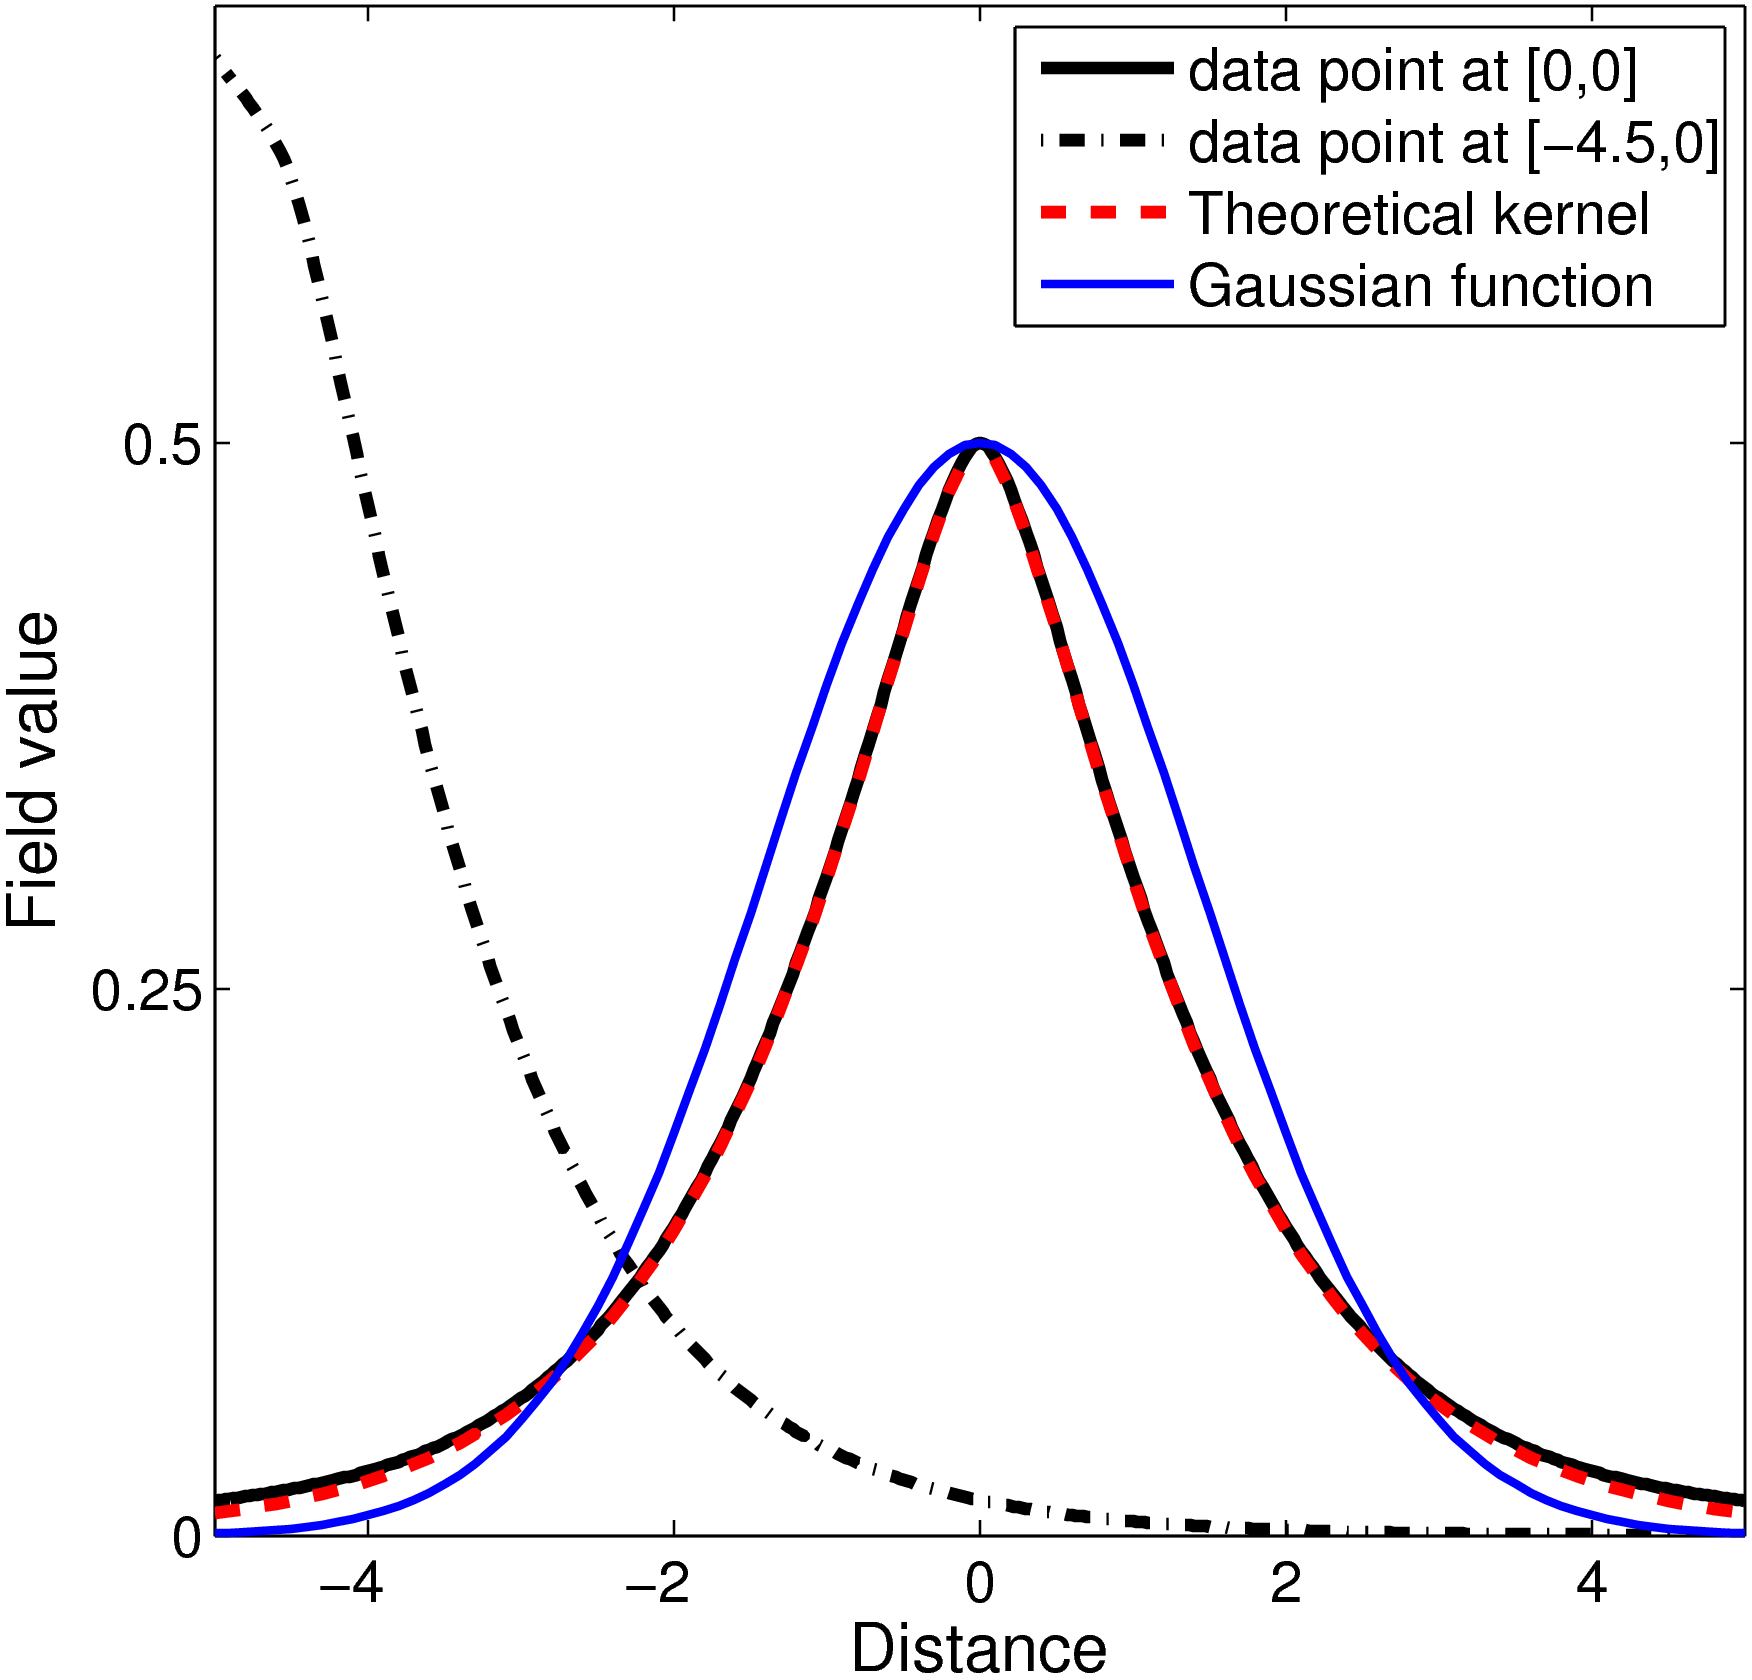
\includegraphics[width=.7\textwidth,bb=66 206 510 630]{fig4_kernel_bceffect}
\caption[Analysis in a square domain with a point at the centre and another at $(-4.5,0)$.]{Analysis in a square domain $[-5,5]\times[-5,5]$ with a point at the centre and another at $(-4.5,0)$. The signal-to-noise ratio $\snr=1$ for both cases. Note the larger analysis value near the boundary, indicating a larger background variance.
\label{fig:fig4_kernel_bceffect}}
\end{figure} 
 
From there, applying the correction $1/(1-\varphi_0)$, we can use the covariances as input vector for a second \diva execution, so as to perform an analysis of the covariance and getting access to the error of the analysis at the desired location. Indeed, using the equivalence of \diva and OI, if the analysis step applied to a data vector $\vect{d}$ is formally written 
\begin{equation}
\varphi_a = \matr{H} \vect{d},
\end{equation}
then the error is 
\begin{equation}
e^2 (\vect{r}) = \sigma^2 \hat{B}(\vect{r},\vect{r}) - \sigma^2 \matr{H} \hat{\vect{b}},
\end{equation}
where $\hat{B}(\vect{r},\vect{r})$ is the local relative background variance (calculated by \eqref{eq:brr}) and $\hat{\vect{b}}$ is a vector filled according to \eqref{eq:btildco}.


\subsubsection{The real covariance method: discussion of background variance\label{sec:backgroundrealcovariance}}


\paragraph{a) Absolute error}


\paragraph{b) Errors scaled by $B_{ii}$}


When relative errors are demanded, one could divide by $\sigma^2 B_{ii}$; 




\paragraph{Discussion}
The effect of spatially non-uniform $B_{ii}$ is particularly clear at the edge of the finite elements grid. If the boundary is in the open ocean, there is actually no reason to suppose that the background error increases when approaching the artificial boundary and dividing by $B_{ii}$ provides a more natural error estimation so that solution b) should be used. 

If near real coasts increased background variance is expected, then the error estimation a) should be used. In such cases, open boundaries should be pushed further away in the numerical finite element grid and the analysis on the regular grid only be done in the region of interest.

\subsection{The almost exact method\label{sec:exerr}}

The idea here is to calcule the error exactly in some selected location and than interpolate the error to provide a gridded error field at a reduced cost. The implementation also allows to avoid the need to run a second diva executable by exploiting an expression of the error at data locations by adding pseudo data in well selected locations.

{\it more to come}

\subsubsection{Background variance}

As for the case of the real covariance, one can select to provide the error scaled by $B_{ii}$ or not.


%-----------------
\section{Usage of methods}
%-----------------

The (clever) poor man's error is useful as a first and quick error field during exploration of data. Once analysis parameters such as correlation length are correctly calibrated, outliers eliminated and the analysis considered relevant, a better error calculation should be used.


Calculation of the full covariance function or the almost exact error version for error calculation is recommended when at least one of the following conditions is true:
\begin{itemize}
\item Advection constraint is strong.
\item Signal-to-noise ratio is high and few data are available near the boundaries.
\item $\xi$ (penalizing gradients) is different from 1 and the kernel is not \eqref{kernelfunction} any more. 
\item The correlation length is variable over the domain. 
\end{itemize}

In the aforementioned cases, the assumptions for the hybrid approach are not fulfilled and the use of \eqref{eq:kernelbessel} to express the covariance will provide an error field that is not coherent with the analysis. For instance, lower errors can be obtained in regions void of observations. 

\section{Numerical cost}

Let us assume that the error is requested at $N_{c}$ locations (sparse points or regular grid). The error computation with OI (in its original formulation) requires the inversion of a matrix of size $N_{d} \times N_{d}$ and the projection of onto the $N_{c}$ locations. We will now see how it can be done with \diva.

\subsection{Poor man's estimate}

An analysis is performed on a vector filled with constant covariance $\sigma^{2}$. As the vector of covariances is filled with identical values $\sigma^{2}$, the error is assessed for all the $N_{c}$ locations with the same analysis. Since the matrix to be inverted for the analysis (the stiffness\index{Stiffness matrix} matrix $\matr{K}$, \eqref{eq:solution}) is already factorized\footnote{$\mathsf{LU}$ decomposition or factorization: the matrix is written as the product of a lower triangular matrix $\mathsf{L}$ and an upper triangular matrix $\mathsf{U}$.}, the additional cost is almost zero because a single analysis is needed.   

\subsection{Hybrid method} 

Again, the cost is kept low by exploiting the already existing factorization. For each of the $N_c$ locations, matrix-vector operations are needed. Roughly, if the cost of the first analysis is $M$, the error field calculation requests $M N_c/\sqrt{N_e}$ operations, where $N_e$ is the number of degrees of freedom of the finite-element mesh.

\subsection{Real covariance function}

For each of the $N_c$ points in which the error is to be evaluated, an additional analyse providing the covariance function is needed. If done naively, this would be prohibitive since a new analyse with another data set (the unit data in different locations) normally requests a new matrix inversion. 

To save computing time, a nice mathematical property was discovered and exploited: performing an analysis that differs only by one data point from a previous analysis can be performed using an already existing matrix factorization. In this case, the generation of all covariances (always changing only one data point) can be performed with a cost similar to a single error analysis with prescribed mathematical covariance functions.

To explain the method, let us suppose that we have constructed and inverted the stiffness matrix\index{Stiffness matrix} $\matr{K_0}$ for the same problem without any data point (as explained in Section~\ref{sec:finiteelements}), $\matr{K_0}$ has a component that is related to the smoothness constraint, not to the data). Then, adding a single data point with unit value at location $i$ would demand the solution of 

\begin{equation}
\left( \matr{K}_0 + \mu_i \matr{S}_i \transp{\matr{S}}_i \right) \vect{q} ~=~ \mu_i \matr{S}_i.
\end{equation}
Here, the \textit{Woodbury-Sherman} formula yields
\begin{equation}
\vect{q}=\left( 1 \over 1 + \mu_i \transp{\matr{S}}_i \inv{\matr{K}}_0 \matr{S}_i \right) \mu_i \inv{\matr{K}}_0 \matr{S}_i.
\label{eq:qwoodone}
\end{equation}
Since the term in parenthesis is a scalar multiplicative factor, the solution with the data is obtained by analysing this data point with the stiffness matrix $\matr{K}_0$ and then multiplying all analyses by $ 1 /( 1 + \mu_i \transp{\matr{S}}_i \inv{\matr{K}}_0 \matr{S}_i)$.
The value of 
\begin{equation} 
\varphi_0 = \mu_i \transp{\matr{S}}_i \inv{\matr{K}}_0 \matr{S}_i
\end{equation}
is actually nothing else than the analysis at the new data location, again using the stiffness matrix $\matr{K}_0$.
Hence the recipe for calculation of the covariances is now clear: 

\begin{enumerate}
\item Create and invert once the stiffness matrix $\matr{K}_0$ constructed without any data points. 
\item For each point for which the covariance is needed:
\begin{enumerate}
\item Create the elementary charge vector $\mu_i \matr{S}_i$.
\item Apply the already inverted stiffness matrix $\inv{\matr{K}}_0$  and the multiplicative factor of \eqref{eq:qwoodone} to derive the values of $\varphi_0$ and $\varphi_i$
\item Compute the covariances using \eqref{eq:brr} and \eqref{eq:btildco}.
\end{enumerate}
\end{enumerate}

The efficiency of the method is due to the fact that we remain within the same \diva execution, where the matrix inversion $\inv{\matr{K}}_0$  is much less expensive than the initial factorization. Indeed the cost is reduced by a factor $\sqrt{N_e}$, with $N_e$ typically around 10$^4$-10$^5$, thus gain is again significant. Each covariance can be stored on disk for later use by the error calculation.

Overall the cost for the full error calculation is now roughly equivalent to twice the hybrid approach, which is a substantial reduction compared to a brute force approach. The only unsolved problem is the storage of the covariance functions if they are calculated before the actual \diva run for the error calculations. This storage will take $N \times N_c$ words when $N_c$ points for error calculations are requested. The intermediate storage can however be avoided by using Unix-pipes between concurrent execution of two \diva cores, one providing the covariance for the other on demand.

%---------------------------------------
\section{Comparison between the methods}
%---------------------------------------


For this application, we employ the same data as in Section~\ref{sec:medseaex} (salinity measurements in the Mediterranean Sea at a depth of 30~m in July, for the 1980-1990 period). Here, the error is scaled locally by the local variance of the background field $\hat{B}$, yielding relative errors. 

The OI field (Fig.~\ref{fig:salinity_error_oi_0707_10030DD}a) shows the effect of the data coverage on the error magnitude. The relative error lies between 40 and 60\% around the regions with a sufficient amount of observations. The largest values ($>80\%$) occur along the south coasts of the Mediterranean Sea, where almost no data are available for the considered period. This means that the analysis obtained in these areas cannot be taken with much confidence.

The poor man's estimate (Fig.~\ref{fig:salinity_error_oi_0707_10030DD}b) provides an error field with lower values over the whole domain. Where data are available, the error is below 20\%, whereas the 80-100\% error region is limited to a small zone close to the coast of Libya. 

%The relation \eqref{eq:erroroi} explains why this method underestimate the error: the error variance ($e^2$) is obtained by subtracting the analysis applied to a vector containing the data covariances ($\matr{H} \vect{c}$) to the variance of the background field ($\signal^2$). When we replace the covariance vector $\vect{c}$ by a vector containing only $1$, the covariances are overestimated, so is the error reduction by the analysis. 

The hybrid method was build by analogy with the OI error estimate \citep{BRANKART98}. Thus it is expected that the two methods provide comparable results. Indeed, the error field of Figs.~\ref{fig:salinity_error_oi_0707_10030DD}(a) and (c) exhibit a similar spatial distribution. Some discrepancies appear in certain regions: along the Italian coasts (on both side of the Peninsula), in the Alboran Sea, and around Cyprus. These differences are related to the presence of the coasts: 
\begin{enumerate}
\item As with the analysis, the FE method prevent the information to cross land. Hence the error reduction due to the analysis is lower with the hybrid method than with OI. 
\item Close to the coasts, the variance of the background field in \diva is increased, due to the specified boundary conditions. 
\end{enumerate}

Finally, the error using the real covariance function (Fig.~\ref{fig:salinity_error_oi_0707_10030DD}d) is also close to the hybrid results. The main differences between the two methods occur in the coastal areas, for instance in the Adriatic Sea or around Cyprus. In these regions, the error is lower when the real covariance is employed, because it allows for the consideration of coastline effects. 


\begin{figure*}[htpb]
\centering
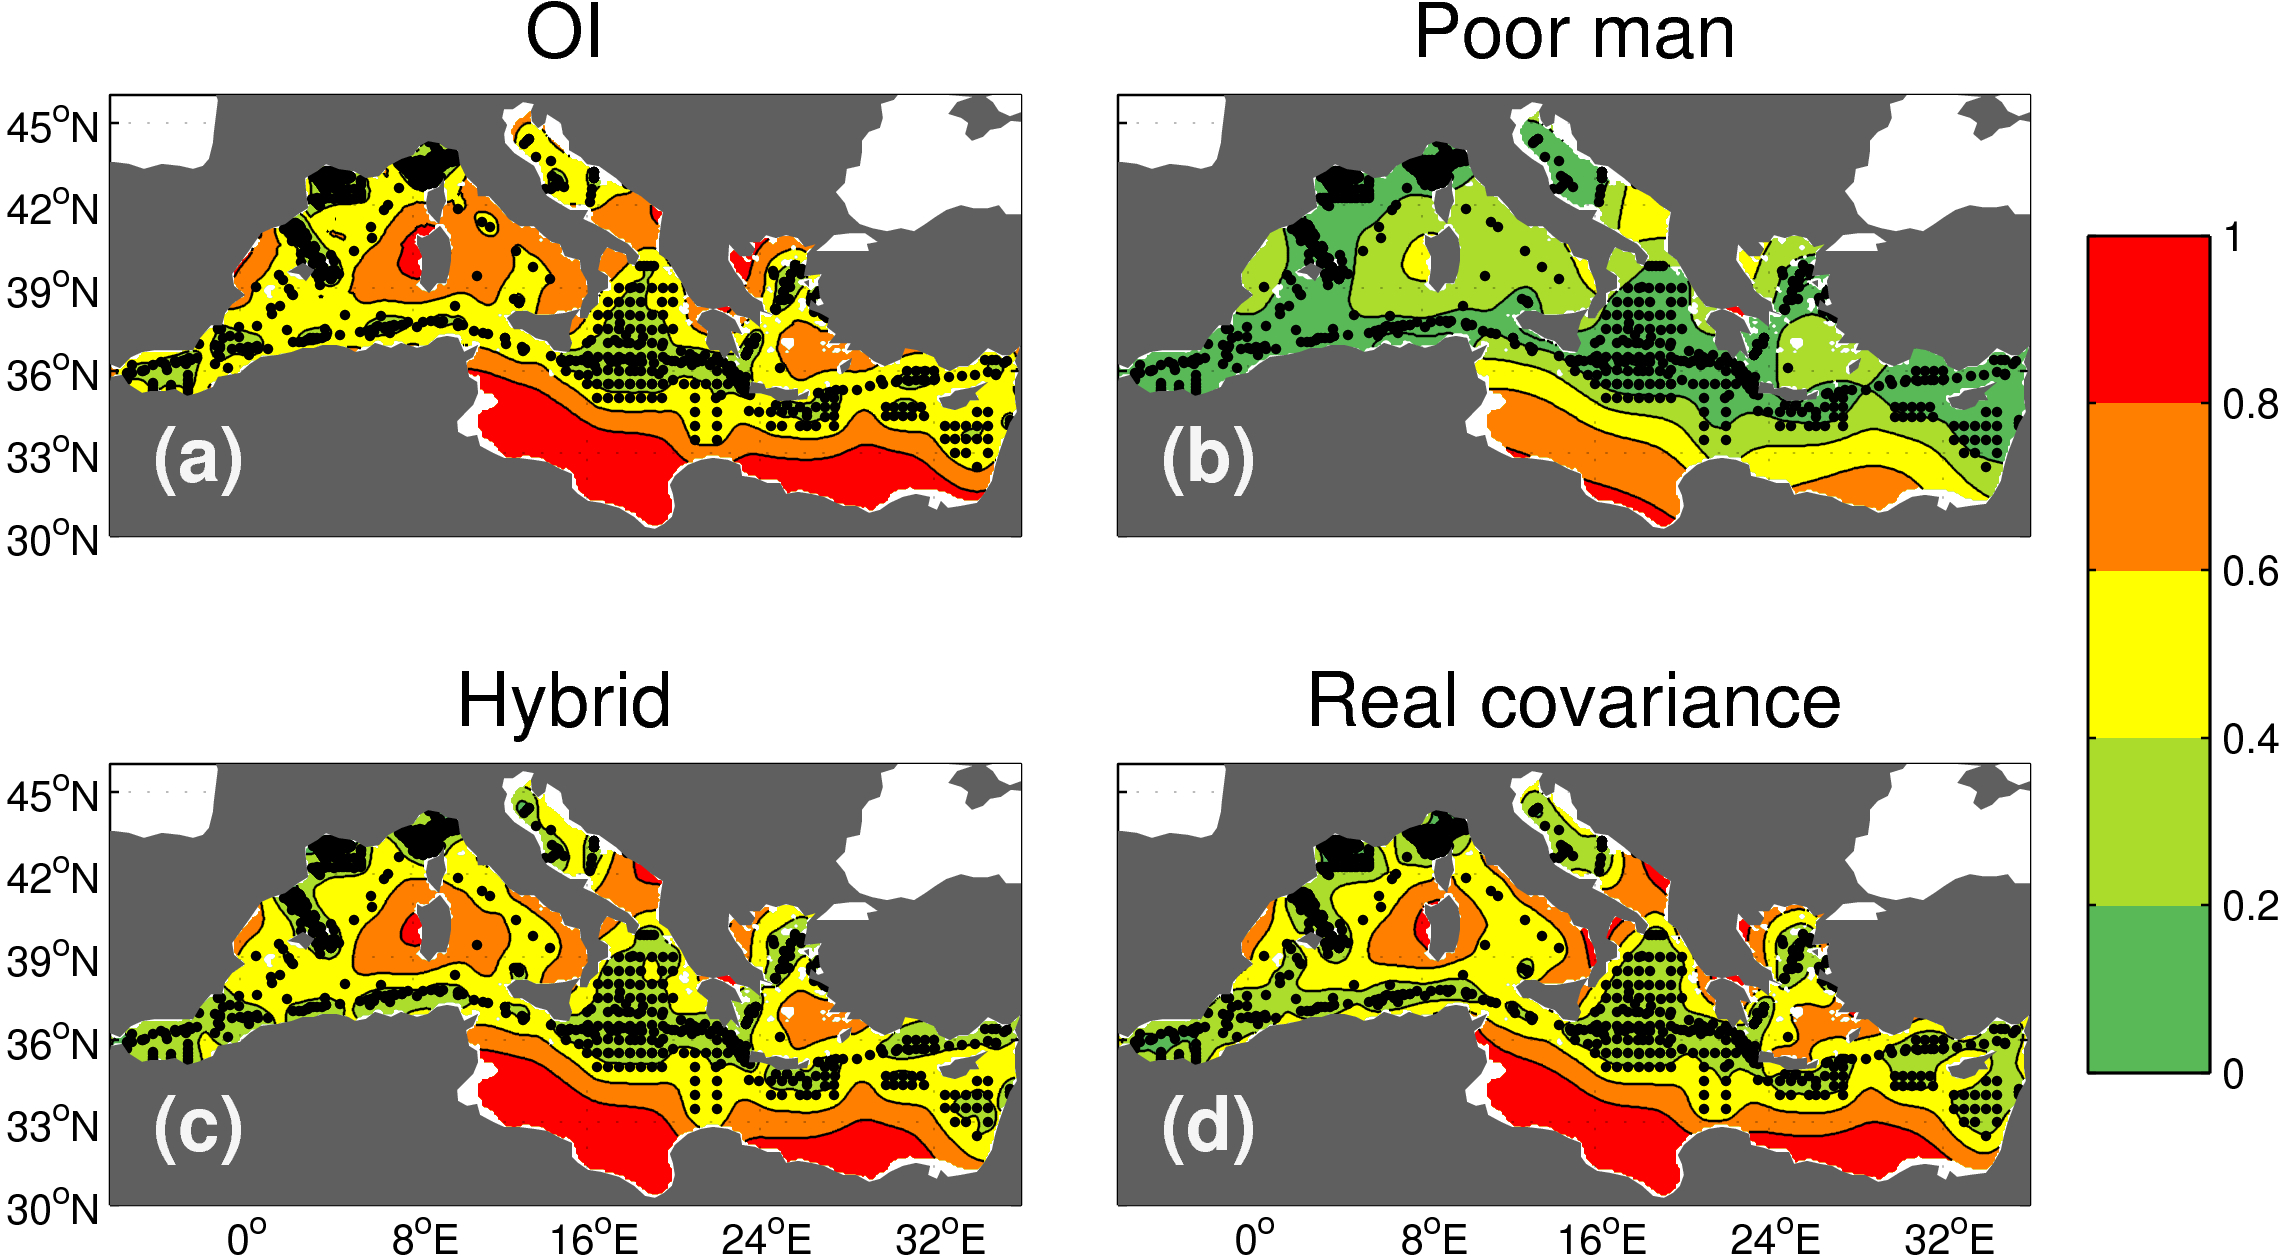
\includegraphics[width=1.35\textwidth,angle=90,bb=24 292 581 605]{salinity_error_oi_0707_10030DD}
\caption[Error fields computed using four different methods.]{Error fields computed using four different methods: (a) OI, (b) poor man's estimate, (c) hybrid and (d) real covariance methods.\label{fig:salinity_error_oi_0707_10030DD}}
\end{figure*}

The choice of one particular method depends on several factors:
\begin{itemize}
\item The size of the output grid.
\item The number of analyses to be performed.
\item The sources of anisotropies (advection, coastlines).
\end{itemize} 

If the objective is limited to having an indication of the area where the analysed field cannot be trusted, then the poor man's estimate is sufficient. If a more complex error field is to be constructed, a bypass is the reduction of the output grid resolution. This solution is particularly welcome when a large number of analyses ($\mathcal{O}(10^{2})$) is required, as it is the case for a climatology (repeated analysis on months and depth levels).


% \section{Error field with advection}

% provided by diva, but interpretation different as the normal case
% need to add more details on this


\clearpage

%------------------------------------
\section{Integrals over (sub-)domains}
%------------------------------------

Very often, we are not only interested in the analysed field itself but also in its integral over the
total domain or a sub-domain. If we have the analysis on a sufficiently fine output grid, the integral
itself is then just a sum of the values at the grid points covering the integration domain, multiplied by the
grid-cell surface. 

We do not consider here the additional approximation brought by replacing a continuous integral by
a discrete sum. Indeed, generally the output grid is fine compared to the scales of interest
and the sum can be considered an "exact" integral. Hence, we will focus on the error on a discrete sum of the analysed field.

An application of this theory is found in \citet{YARI12}, where the authors estimated transports through the Strait of Otranto (Adriatic Sea) using \diva and the calculation of integrals.

\subsection{Theory}
%------------------

Formally, if $\mathbf{x}^a$ is a column vector containing the analysed field values at the grid
points defining the integration domain, the weighted sum $I$ over this values is
\begin{equation}
I~=~\transp{(\mathbf{x}^a)} \mathbf{h}
\end{equation}
where $\transp{\quad}$ stands for the transposed vector or matrix and $\mathbf{h}$ is a column vector of the same size as
$\mathbf{x}^a$ but whose components are the weight associated with each integration point. The weight is typically the surface associated with
the integration point. For an integration over a uniform grid, the weights can without loss of generality be unit (the surface dimension can be retrieved at the end by global multiplication). 

Note that the weights here have nothing to do with the weight on data points for an analysis\index{Weight}.

Now the analysis is not exact but has an associated random error $\mathbf{\epsilon}^a$ with respect to the true
field values $\mathbf{x}^t$:

\begin{equation}
{\mathbf{x}^a} = \mathbf{x}^t + \mathbf{\epsilon}^a
\end{equation}
On statistical average (noted $< \quad >$), we suppose the analysis is unbiased and
\begin{equation}
<{\mathbf{x}^a}> = \mathbf{x}^t 
\end{equation}
In order to calculate the error variance on the sum, we calculate the expected square distance with respect to the true sum:
\begin{equation}
\Delta^2 = < \transp{\mathbf{h}}( {\mathbf{x}^a} - \mathbf{x}^t) \transp{({\mathbf{x}^a} - \mathbf{x}^t )} \mathbf{h} > = \transp{\mathbf{h}} \, \mathbf{P}^a \, \mathbf{h}
\label{eq:errorintegral}
\end{equation}
where $\mathbf{P}^a = <\mathbf{\epsilon}^a \transp{\mathbf{\epsilon}^a} >$ is the error-covariance matrix of the analysis.
We see that the spatial covariances of the analysis-error field are required to calculate the error variance on $I$. Since this
covariance matrix is not diagonal, it is not sufficient to sum up the local error values of the error fields of $\mathbf{x}^a$. The latter sum would limit
the double sum of \eqref{eq:errorintegral} to the diagonal terms of $\mathbf{P}^a$.


\subsection{Implementation}
Exploiting the equivalence of \diva and OI, we know that

\begin{equation}
\mathbf{P}^a ~=~ \mathbf{P} -  \transp{\mathbf{C}} \left( \mathbf{B}+\mathbf{R} \right)^{-1} \mathbf{C}
\label{eq:covariance}
\end{equation}
where $\mathbf{P}$ is the covariance matrix (size $N_g\times N_g$) of the background field between the $N_g$ grid points under consideration, $\mathbf{B}$ 
the covariance matrix (size $N_d \times N_d$) of the background field between the $N_d$ data points, $\mathbf{C}$  is the
 covariance matrix (size $N_d \times N_g$) of the background field between the  data points and grid points and finally $\mathbf{R}$ is the error covariance matrix (size $N_d \times N_d$) on the data.
 
We could calculate the covariances matrices involved exactly (as done for the exact error calculation) and then calculate \eqref{eq:errorintegral} but this would be prohibitively expensive if done in a brute force approach. However when done in a clever way it is feasible.

\subsubsection{Direct approach}

Using \eqref{eq:covariance} and \eqref{eq:errorintegral} we can write

 \begin{equation}
 \Delta^2 = \transp{\mathbf{h}}\, \mathbf{P} \, \mathbf{h} - \transp{\mathbf{h}} \underbrace{\transp{\mathbf{C}} \left( \mathbf{B}+\mathbf{R} \right)^{-1}} \, \underbrace{\mathbf{C}  \, \mathbf{h}}
 \label{eq:totalerror}
 \end{equation}
 
The term $\mathbf{C}  \, \mathbf{h}$ is readily interpreted as a columns vector containing $N_d$ elements. Element $j$ is the (weighted) sum of the covariances of all integration points with the data point $j$. The middle term is the analysis operator that provides the analysis on the grid points when providing on input a columns vector of size $N_d$. Hence the recipe to calculate $\Delta^2$ without explicitly forming the error-covariance matrices is the following:
\begin{itemize}
\item Perform a double sum on all covariances between grid points to calculate $\transp{\mathbf{h}} \, \mathbf{P} \, \mathbf{h}$.
\item For the term to subtract, evaluate it starting from the right: form a pseudo-data vector by summing covariances of all grid points with each data point, analyse it and finally sum up the analysis at the grid points.
\end{itemize}

All we have to to is to be calculate covariance functions. This can be done with the module {\tt covar} of \diva, which allows one to calculate
a series of covariances with a single matrix inversion. Hence the recipe of calculating \eqref{eq:totalerror} includes a \diva run to calculate covariances (cost roughly equal to an analysis with full error field), followed by a second \diva run to analyse the "data" $\mathbf{C}  \, \mathbf{h}$.



\subsubsection{Hybrid approach}

A simplified version can be used, using to some extend the fact the covariance functions in an infinite domain are known analytically when no
advection constraint or variable correlation length is activated. We can indeed introduce an approximation that makes the calculation manageable without calculating the covariances with \diva itself. Instead of using the exact covariances on the background field, we use the covariances we would find in an infinite domain with constant correlation length and without advection constraint. In this case, we know
that the correlation function $c$ between two points is
\begin{equation}
c(r) ~=~{r \over L} K_1 \left(r \over L\right)
\end{equation}
where $r$ is the distance between the two points, $L$ the correlation length and $K_1$ a Bessel function\index{Bessel function}. To get the covariance function we simply have to multiply by the variance $\sigma^2$ of the background field.

This way we can estimate $\Delta^2$ by calculating these covariance functions between grid and data points and performing one analysis with \diva.

\subsubsection{Inflation approach}

A second simplified approach makes even stronger assumptions but shows how we can try to "extrapolate" the error estimated from the sum of the diagonal terms of $\mathbf{P}^a$ to the estimation of the double sum. To do so, we assume that the analysis error has a spatial correlation scale similar to the analysis.
This is probably too severe and we will therefore overestimate the integral error. 
Here we use a continuous formulation to calculate an approximation of $\Delta$ noted $\tilde{\Delta}$ by starting from the sum expressed as continuous integral
\begin{equation}
{\Delta}^2= {1 \over \Delta x^2 \Delta y^2} \int_D \int_D <{\epsilon}^a(\vect{x}) {\epsilon}^a(\vect{x}^\prime)> d \vect{x}^\prime d \vect{x} 
\end{equation}
where $\vect{x}$ and $\vect{x}^\prime$ stand for positions in the domain of integration $D$. When we suppose the covariance is isotropic and note $r$ the distance between points
$\vect{x}$ and $\vect{x}^\prime$ we have 
\begin{equation}
{\Delta}^2= {1 \over \Delta x^2 \Delta y^2} \int_D \int_D <{\epsilon}^a(\vect{x}) {\epsilon}^a(\vect{x}) > c(r) d \vect{x}^\prime d \vect{x}  
\end{equation}
which we can evaluate in polar coordinates the inner integral expanded to infinity to find an approximate value
\begin{equation}
\tilde{\Delta}^2= {2 \pi \over \Delta x^2 \Delta y^2} \int_D <{\epsilon}^a(\vect{x}) {\epsilon}^a(\vect{x}) > \int_0^{\infty}  r c(r) d r \, d \vect{x}
\end{equation}
with the Bessel function for the correlation function $c$ this yields
\begin{equation}
\tilde{\Delta}^2= {4 \pi L^2 \over \Delta x^2 \Delta y^2} \int_D <{\epsilon}^a(\vect{x}) {\epsilon}^a(\vect{x}) >  d \vect{x}
\end{equation}

If we had used the naive approach of neglecting the spatial covariances, the double sum would have been restricted to a simple sum on diagonal and we would calculated the underestimated error 
\begin{equation}
\tilde{\tilde{\Delta}}^2= {1 \over \Delta x \Delta y} \int_D <{\epsilon}^a(\vect{x}) {\epsilon}^a(\vect{x}) >  d \vect{x}.
\end{equation}
Hence we see that we should apply an inflation factor of $\sqrt{{4 \pi L^2 \over \Delta x \Delta y}}$ on $\tilde{\tilde{\Delta}}$ to get a better estimate of the error standard deviation. In practice this inflation factor is probably a little too high (we assumed the analysis error to have the same correlation length as the analysis while in reality it is generally smaller and we extended one of the integrals to an infinite domain, adding up more errors).

\subsection{Use}

All approaches were implemented into \command{divaintegral}. If there is a file\\ 
\file{./input/integrationpoints.dat}, it will be used.
Otherwise it will be created (and put in the \directory{./output}), based on the analysis on the output grid. This files must contain \texttt{x,y,val,1,h}. If the file did not exist but was created, it will pass through an execution of \command{divaintegral}. 
\command{divaintegral} can be edited by the user to chose special points for the integration (for example only those points for which the analysis is positive, or points that fall in a given square etc). 

When {\tt ispec } is negative, the full covariance calculation will be used. When {\tt ispec} is positive, the hybrid covariance calculation will be used.

When called with the optional argument \texttt{-naive}, it also calculates the simple sum of the diagonal term of the analysis error variance. The error field itself is calculated with the methods specified by \texttt{ispec}. 

\begin{lstlisting}[style=Bash]
[charles@gher13 divastripped] divaintegral -naive
\end{lstlisting}

The output files generated are:
\begin{itemize}
\item \file{./output/integral.dat} contains the integral value, the surface of the integration domain and the average value (integral divided by surface).
\item \file{./output/erroronintegral.dat} contains the error standard deviation on the integral, in the same units as the integral.
\item \file{./output/erroronintegralnaive.dat} contains the naive approach summing only the diagonal terms, the inflation factor and the inflated error. Units are the same as the integral.
\end{itemize}

Units are units of the variable multiplied by the units of $x$ and $y$ of the data and contour file, when no coordinate change is performed or the option {\tt icoordchange = -xscale} was used.

When {\tt icoordchange} is one or two, the surface units of the output are m$^2$.

Note that the tool is not designed for use with the poor man's error calculation (\texttt{ispec}>10, Section~\ref{sec:poormans}).

\subsection{Interna}
%-------------------

\begin{itemize}

\item \texttt{gridpointlist.a} creates a list of wet points of the analysis grid. 

Input: \file{fort.20} gridded gher file, \file{fort.21} corresponding to \file{GridInfo.dat}.\\ 
Output: \file{fort.22} list of points with value of analysis on wet points only (\texttt{x,y,val,1,1}).

\item \texttt{erroronintegrals.a} calculates the double sum on background covariance and prepares the pseudo-data (sum of covariances of all grid points with a  data point).

Input: \file{fort.10} list of grid points for the integral (including third column for value of field), \file{fort.11} data file, \file{fort.5} with \texttt{scale lc datacol}.\\
Output: \file{fort.14} double sum, \file{fort.12} pseudo-data vector.
\end{itemize}

For exact covariance functions, 

\begin{lstlisting}[style=Bash]
[charles@gher13 divastripped] divacalc -pfsum
\end{lstlisting}

is executed, which allows the use of the full suite of \diva parameters (including for example advection constraint). Internally, as we need the covariance of all integral points with all integral points and data locations, we provide to \command{divacalc -pfsum} in input "data" which are the integration points and ask in addition values in a list of points (which are the original data location).

